% -*- mode: tex; fill-column: 115; -*-

\documentclass[a4paper, twoside]{article}
\setcounter{secnumdepth}{5}
\setcounter{tocdepth}{5}
\usepackage[english]{babel}
\usepackage{textcomp}
\usepackage{amsmath,amsthm,amsfonts,amssymb,epsfig}
\usepackage{array}
\usepackage{datetime}
\usepackage{lipsum}% http://ctan.org/pkg/lipsum
\usepackage[left=1.1in,top=1in,right=1.1in]{geometry}% http://ctan.org/pkg/geometry
\usepackage{listings}% http://ctan.org/pkg/listings
\usepackage{spverbatim}
\usepackage{hyperref}
\usepackage{microtype}
\hypersetup{colorlinks=true, urlcolor=black, linkcolor=black}
\usepackage{graphicx}
\graphicspath{ {images/} }
\usepackage{parskip}
\usepackage{titlesec} %used for diminishing heading sizes
\usepackage[square, sort, comma, numbers]{natbib} %%uses titles for cited references
\usepackage[fit]{truncate}
\usepackage{fancyhdr}
\pagestyle{fancy}
\fancyhead{}
\fancyhead[RO, RE]{\thepage}
\fancyhead[LO, LE]{\rightmark}
\renewcommand{\sectionmark}[1]{\markboth{}{\textsc{\thesection~#1}}}
\fancyfoot[C]{}%hide footer
\usepackage{xcolor} 
\usepackage[scaled=1]{couriers}

\xdefinecolor{gray}{rgb}{0.6,0.6,0.6} 

\defcitealias{glmnet}{Regularization Paths for Generalized Linear Models via Coordinate Descent by Friedman et. al}
\defcitealias{strong}{Strong Rules for Discarding Predictors in Lasso-type Problems by Bien et. al}
\defcitealias{admm}{Distributed Optimization and Statistical Learning via the Alternating Direction Method of Multipliers by Boyd et. al}
\defcitealias{prox}{Proximal Algorithms by Boyd et. al}


\titleformat*{\section}{\LARGE\bfseries\sffamily}
\titleformat*{\subsection}{\Large\bfseries\sffamily}
\titleformat*{\subsubsection}{\large\bfseries\sffamily}
\titleformat*{\paragraph}{\large\bfseries\sffamily}
\titleformat*{\subparagraph}{\large\bfseries\sffamily}
\renewcommand{\familydefault}{\sfdefault} %sans-serif font



\begin{document}


%----------------------------------------------------------------------
% Definition for "lstlisting" blocks
%----------------------------------------------------------------------
% --- USAGE ---
%
% \begin{lstlisting}[style=R}
% ...
% \end{lstlisting}
%
% % \begin{lstlisting}[style=output}
% ...
% \end{lstlisting}
%----------------------------------------------------------------------

% By default, make listings all black so it's easy to spot the ones that aren't set to a style.
% This is just a debugging technique.
\lstset{backgroundcolor=\color{black}}

% Define scala language first
% ``define'' Scala
\lstdefinelanguage{scala}{
  morekeywords={abstract,case,catch,class,def,%
    do,else,extends,false,final,finally,%
    for,if,implicit,import,match,mixin,%
    new,null,object,override,package,%
    private,protected,requires,return,sealed,%
    super,this,throw,trait,true,try,%
    type,val,var,while,with,yield},
  otherkeywords={=>,<-,<\%,<:,>:,\#,@},
  sensitive=true,
  morecomment=[l]{//},
  morecomment=[n]{/*}{*/},
  morestring=[b]``,
  morestring=[b]',
  morestring=[b]''``
}

\lstdefinestyle{R}{
  language=R,
  frame=single,
  breaklines,
  basicstyle=\ttfamily,
  commentstyle=\textbf,% comment style
  keywordstyle=\ttfamily,
  numbers=left,% display line numbers on the left side 
  numberstyle=\scriptsize,% use small line numbers 
  numbersep=10pt,% space between line numbers and code
  backgroundcolor=\color{white}, 
  showstringspaces=false % don't show spaces as weird char.
}

\lstdefinestyle{python}{
  language=python,
  frame=single,
  breaklines,
  basicstyle=\ttfamily,
  commentstyle=\textsl,% comment style
  keywordstyle=\ttfamily,
  numbers=left,% display line numbers on the left side 
  numberstyle=\scriptsize,% use small line numbers 
  numbersep=10pt,% space between line numbers and code
  backgroundcolor=\color{white}, 
  showstringspaces=false %don't show spaces as weird char.
}

\lstdefinestyle{Scala}{
  language=scala,
  frame=single,
  breaklines,
  basicstyle=\ttfamily,
  commentstyle=\textsl,% comment style
  keywordstyle=\ttfamily,
  numbers=left,% display line numbers on the left side 
  numberstyle=\scriptsize,% use small line numbers 
  numbersep=10pt,% space between line numbers and code
  backgroundcolor=\color{white}, 
  showstringspaces=false % don't show spaces as weird char.
}

\lstdefinestyle{Bash}{
  language=bash,
  frame=single,
  breaklines,
  basicstyle=\ttfamily,
  commentstyle=\textsl,% comment style
  keywordstyle=\ttfamily,
  numbers=left,% display line numbers on the left side 
  numberstyle=\scriptsize,% use small line numbers 
  numbersep=10pt,% space between line numbers and code
  backgroundcolor=\color{white}, 
  showstringspaces=false % don't show spaces as weird char.
}


\definecolor{mygray}{rgb}{0.92,0.92,0.92}

\lstdefinestyle{output}{
  frame=single,
  breaklines,
  basicstyle=\ttfamily,
  numbers=left,% display line numbers on the left side 
  numberstyle=\scriptsize,% use small line numbers 
  numbersep=10pt,% space between line numbers and code
  backgroundcolor=\color{mygray}, 
  showstringspaces=false %don't show spaces as weird char.
}

\newcommand{\waterExampleInR} {
\textbf{Example in R} \\
}

\newcommand{\waterExampleInPython} {
\textbf{Example in Python} \\
}


\thispagestyle{empty} %removes page number

\begin{center}
\textsc{\Large\bf{Generalized Linear Modeling with H2O}}
\\
\bigskip
\textsc{\small{Tomas Nykodym \hspace{20pt} Ariel Rao \hspace{20pt} Amy Wang \hspace{20pt} Tom Kraljevic \hspace{20pt} Jessica Lanford}}
\\
\bigskip
\line(1,0){250}  %inserts  horizontal line

\bigskip
August 2015: Third Edition 
\\%add front page image here? (wavy lines)
\bigskip
\end{center}

{\raggedright\vfill\ 

Generalized Linear Modeling with H2O\\
  by Tomas Nykodym, Ariel Rao, Amy Wang, Tom Kraljevic, \&\ Jessica Lanford \\
\bigskip
  Published by H2O.ai, Inc. \\
2307 Leghorn St. \\
Mountain View, CA 94043\\
\bigskip
\textcopyright 2015 H2O.ai, Inc. All Rights Reserved. 
\bigskip

August 2015: Third Edition
\bigskip

Photos by \textcopyright H2O.ai, Inc.
\bigskip

While every precaution has been taken in the\\
preparation of this book, the publisher and\\
authors assume no responsibility for errors or\\
omissions, or for damages resulting from the\\
use of the information contained herein.\\
\bigskip
Printed in the United States of America. 
}

\newpage

\tableofcontents

%----------------------------------------------------------------------
%----------------------------------------------------------------------

\newpage

\section{Introduction}
This document introduces the reader to Generalized Linear Modeling with H2O.  Examples are written in R and python.
The reader is walked through the installation of H2O, basic GLM concepts, building GLM models in H2O, how to
interpret model output, how to make predictions, and various implementation details.

%----------------------------------------------------------------------
%----------------------------------------------------------------------

\section{What is H2O?}
\Urlmuskip=0mu plus 1mu\relax %needed to make long URLs break nicely


H2O is fast, scalable, open-source machine learning and deep learning for smarter applications. With H2O, enterprises like PayPal, Nielsen Catalina, Cisco, and others can use all their data without sampling to get accurate predictions faster. Advanced algorithms such as deep learning, boosting, and bagging ensembles are built-in to help application designers create smarter applications through elegant APIs. Some of our initial customers have built powerful domain-specific predictive engines for recommendations, customer churn, propensity to buy, dynamic pricing, and fraud detection for the insurance, healthcare, telecommunications, ad tech, retail, and payment systems industries.

Using in-memory compression, H2O handles billions of data rows in-memory, even with a small cluster. To make it easier for non-engineers to create complete analytic workflows, H2O's platform includes interfaces for R, Python, Scala, Java, JSON, and CoffeeScript/JavaScript, as well as a built-in  web interface, Flow. H2O was built alongside (and on top of) Hadoop and Spark Clusters and typically deploys within minutes.

H2O includes many common machine learning algorithms, such as generalized linear modeling (linear regression, logistic regression, etc.), Na\"{i}ve Bayes, principal components analysis, time series, k-means clustering, and others. H2O also implements best-in-class algorithms at scale, such as distributed random forest, gradient boosting and deep learning. Customers can build thousands of models and compare the results to get the best predictions.

H2O is nurturing a grassroots movement of physicists, mathematicians, and computer scientists to herald the new wave of discovery with data science by collaborating closely with academic researchers and Industrial data scientists. Stanford university giants Stephen Boyd, Trevor Hastie, Rob Tibshirani advise the H2O team on building scalable machine learning algorithms. With hundreds of meetups over the past three years, H2O has become a word-of-mouth phenomenon, growing amongst the data community by a hundred-fold, and is now used by 30,000+ users and is deployed using R, Python, Hadoop, and Spark in 2000+ corporations.

\textbf{Try it out}

\begin{itemize}
\item  Download H2O directly at \mbox{\url{http://h2o.ai/download}}.
\item Install H2O's R package from CRAN at {\url{https://cran.r-project.org/web/packages/h2o/}}. 
\item Install the Python package from PyPI at {\url{https://pypi.python.org/pypi/h2o/}}.

\end{itemize}



\textbf{Join the community}
\begin{itemize}
\item  To learn about our meetups, training sessions, hackathons, and product updates, visit {\url{http://h2o.ai}}. 
\item Visit the open source community forum at {\url{https://groups.google.com/d/forum/h2ostream}}.
\item Join the chat at {\url{https://gitter.im/h2oai/h2o-3}}.
\end{itemize}





%----------------------------------------------------------------------
%----------------------------------------------------------------------

\newpage

%\subsubsection{Summary of features} 
%In summary, H2O's GLM functionalities include:
%
%\begin{itemize} 
%\item automatic standardization of predictor variables
%\item fits generalized linear model with elastic net penalty
%\item supported GLM families include Gaussian, Binomial, Poisson, Gamma, and Tweedie
%\item efficient handling of categorical variables
%\item efficient computation of full regularization path
%\item IRLSM (best for data with many rows and fewer predictors) and LBFGS (best for data with many predictors) solvers
%\item automatic lambda search for best model
%\item stopping criterium when many predictors are used
%\item efficient distributed n-fold cross validation
% \item distributed grid search over elastic-net parameter $\alpha$
%\item offset column
%\item row weights
%\item upper and lower bounds for coefficients
%\item proximal operator interface
%\end{itemize}

\newcommand{\waterVersion}{3.0.1.4}
\section{Installation} 
\Urlmuskip=0mu plus 1mu\relax %needed to make long URLs break nicely


The easiest way to directly install H2O is  via an R or Python package.

({\bf{Note}}: The examples in this document were created with H2O version \waterVersion.)

\subsection{Installation in R}

To load a recent H2O package from CRAN, run:

\begin{lstlisting}[style=R]
install.packages("h2o")
\end{lstlisting}

{\bf{Note}}: The version of H2O in CRAN is often one release behind the current version.

For the latest recommended version, download the
latest stable H2O-3 build from the H2O download page:

\begin{enumerate}
\item Go to {\url{http://h2o.ai/download}}.
\item Choose the latest stable H2O-3 build.
\item Click the ``Install in R'' tab.
\item Copy and paste the commands into your R session.
\end{enumerate}

\bigskip
After H2O is installed on your system, verify the installation:

\begin{lstlisting}[style=R]
library(h2o)

#Start H2O on your local machine using all available cores.
#By default, CRAN policies limit use to only 2 cores.
h2o.init(nthreads = -1)

#Get help
?h2o.glm
?h2o.gbm

#Show a demo
demo(h2o.glm)
demo(h2o.gbm)
\end{lstlisting}

\subsection{Installation in Python}

To load a recent H2O package from PyPI, run:

\begin{lstlisting}[style=python]
pip install h2o
\end{lstlisting}

To download the
latest stable H2O-3 build from the H2O download page:

\begin{enumerate}
\item Go to {\url{http://h2o.ai/download}}.
\item Choose the latest stable H2O-3 build.
\item Click the ``Install in Python'' tab.
\item Copy and paste the commands into your Python session.
\end{enumerate}

\bigskip
After H2O is installed, verify the installation:

\begin{lstlisting}[style=python]
import h2o

# Start H2O on your local machine
h2o.init()

# Get help
help(h2o.glm)
help(h2o.gbm)

# Show a demo
h2o.demo("glm")
h2o.demo("gbm")

\end{lstlisting}

\subsection{Pointing to a Different H2O Cluster}

The instructions in the previous sections create a one-node H2O cluster on your local machine. 

To connect to an established H2O cluster (in a multi-node Hadoop environment, for example) specify the IP address and port number for the established cluster using the \texttt{ip} and \texttt{port} parameters in the \texttt{h2o.init()} command.  The syntax for this function is identical for R and Python:
\medskip  

\begin{lstlisting}[style=R]
h2o.init(ip = "123.45.67.89", port = 54321)
\end{lstlisting}

%if it's the same, only one is needed



\section{GLM Concepts}
Generalized linear models (GLM) are the workhorse for most predictive analysis use cases. GLM can be used for both
regression and classification, it scales well to large datasets, and is based on solid statistical background. It
is a generalization of linear models, allowing for modeling of data with exponential distributions and for
categorical data (classification). GLM models are fitted by solving the maximum likelihood optimization problem.

Generalized linear models are generalizations of linear regression models. Linear regression models the dependency
of response y on a vector of predictors x ($y \sim x^T \beta + \beta_0$). The models are built with the assumptions
that y has a gaussian distribution with a variance of $\sigma^2$ and the mean is a linear function of x with an
offset of some constant $\beta_0$, i.e. $ y = \mathcal{N}(x^T \beta + \beta_0 , \sigma^2) $. These assumptions can
be overly restrictive for real-world data that do not necessarily have a gaussian distribution.

GLM generalizes linear regression in the following ways: 

\begin{itemize} 
\item adding a non-linear link function that transforms the expectation of response variable, so that $link(y) \sim x^T \beta + \beta_0$.
\item allowing variance to depend on the predicted value by specifying the conditional distribution of the response variable or the family argument.
\end{itemize}

This generalization allows us to use GLM on problems such as binary classification (also known as logistic regression).

\subsection{GLM in H2O}
H2O's GLM algorithm fits the generalized linear model with elastic net penalties. The model fitting computation is
distributed, extremely fast, and scales extremely well for models with a limited number ($\mathtt{\sim}$ low
thousands) of predictors with non-zero coefficients. The algorithm can compute models for a single value of a
penalty argument or the full regularization path, similar to the glmnet package for R (refer
to \citetalias{glmnet}).  H2O's GLM fits the model by solving following problem:

\[ \min\limits_{\beta}\ (\ Classic GLM  + Regularization Penalty \ )\]

which is equivalent to:

\[ \min\limits_{\beta}\ (\ {{1\over{N}} log\_likelihood(family,\beta)  + \lambda (\alpha \| \beta \|_1} + {1- \alpha \over 2} \| \beta \|_2^2) \ )\]

\bigskip
The elastic net parameter $\alpha$ controls the penalty distribution between L1 (Lasso) and L2 (Ridge Regression)
penalties. The range is any value between 0 and 1. When $\alpha$ = 0, we have no L1 penalty and the problem becomes
ridge regression. If $\alpha$ = 1, there is no L2 penalty and we have lasso.

The main advantage of an L1 penalty is that with sufficiently high $\lambda$, it produces a sparse solution; the
L2-only penalty does not reduce coefficients to exactly 0. The two penalties also differ in the case of correlated
predictors. The L2 penalty shrinks coefficients for correlated columns towards each other, while the L1 penalty
will pick one and drive the others to zero. Using the elastic net argument $\alpha$, you can combine these two
behaviors. It is also useful to always add a small L2 penalty to increase numerical stability.

Similarly to the methods discussed in \citetalias{glmnet}, H2O can compute the full regularization path, starting
from null-model (maximum penalty) going down to minimally penalized model. This search is made efficient by
employing strong-rules as described in \citetalias{strong} to filter out inactive coefficients (coefficients pushed
to zero by penalty). Computing the full regularization path is useful in that it gives more insight about the
importance of individual coefficients and quality of the model while allowing selection of the optimal amount of
penalization for the given problem and data.

\subsection{Model Fitting}
GLM models are fitted by maximizing the likelihood. For the gaussian family, maximum likelihood is simply the
minimal mean squared error, which has an analytical solution and can be solved with ordinary least squares. For all
other families, the maximum likelihood problem has no analytical solution so we must use an iterative method such
as IRLSM, Newton method, gradient descent, or L-BFGS.

\subsection{Model Validation}
Evaluating the quality of the model is a critical part of any data-modeling and scoring process. There are several
standard ways to evaluate the quality of the fitted GLM model; the most common method is to use the resulting
deviance. Deviance is calculated by comparing the log likelihood of the fitted model with log likelihood of the
saturated model (or theoretically perfect model).

\[ deviance = 2({ln(L_{s})} - {ln(L_{m})}) \]

Another metric frequently used for model selection is the Akaike information criterion (AIC). The AIC measures the
relative quality of a statistical model for a given set of data obtained by calculating the information loss after
replacing the original data with the model itself. Unlike deviance, which would assign a perfect value for the
saturated model and measures the absolute quality of the fit with a comparison against the null-hypothesis, AIC
takes into account the complexity of the given model. AIC is defined as follows:

\[ aic = 2(k - ln(L_{m}))\]

where k is the number of model parameters and $ln(L_{m})$ is the log likelihood of the fitted model over the data.

\subsection{Regularization} \label{regularization}
We introduce penalties to the model building process to avoid over-fitting, reduce variance of the prediction
error, and handle correlated predictors. There are two common penalized linear models: ridge regression and
lasso. Ridge regression provides greater numerical stability and is easier and faster to compute. In comparison,
lasso leads to a sparse solution, which is advantageous in many situations, as it can be used for feature selection
and to produce models with fewer parameters. When encountering highly correlated columns, the L2 penalty tends to
push all of the coefficients towards each other, while the L1 penalty will pick one and remove the others to
produce 0 coefficients.

\subsubsection{Lasso and Ridge Regression}

Lasso represents the L1 penalty and is an alternative regularized least squares method that uses the constraint
$||B||_1$. The penalty is configured using the \texttt{alpha} parameter. The main difference between lasso and
ridge regression is that as the penalty for ridge regression increases, the parameters are reduced to non-zero
values. With lasso, if the penalty is increased, the parameters can be reduced to zero values. Since reducing
parameters to zero removes them from the model, the lasso method provides only the relevant data. Ridge regression
never removes any data.

\subsubsection{Elastic Net Penalty}

H2O supports elastic net regularization which is parametrized by \texttt{alpha} and \texttt{lambda} arguments
(similar to \citetalias{glmnet})

The \texttt{alpha} argument controls the elastic net penalty distribution to L1 and L2 norms. It can have any value
in the [0,1] range (inclusive) or a vector of values (triggers grid search). If \texttt{alpha = 0}, the result
is \textbf{Ridge Regression}, while if \texttt{alpha = 1} the result is \textbf{LASSO}.

The \texttt{lambda} argument controls the penalty strength; the range is any positive value or a vector of values
(which triggers grid search).

\textbf{Note:} Lambda values are capped at $\lambda_{max}$, which is the smallest $\lambda$ s.t. the solution is
empty model (all zeros except for intercept).

Elastic net combines the two and adds another parameter, $\alpha$, which controls the distribution of the penalty
between L1 and L2. The combination of the two penalties is beneficial, since L1 gives sparsity while L2 gives
stability and encourages the grouping effect (where a group of correlated variables tends to be dropped or added
into the model all at once). One possible use of the $\alpha$ argument is for lasso with very little L2 penalty
($\alpha$ almost 1) to stabilize the computation and improve convergence speed.

A model-fitting problem with an elastic net penalty becomes:

\[ \min\limits_{\beta,\beta_0}\ {{1\over{N}} ln(L(family,\beta,\beta_0))  + \lambda (\alpha \| \beta \|_1}  + {1- \alpha \over 2} \| \beta \|_2^2) \]

\subsection{GLM Model Families}
The following subsection describes the GLM families supported in H2O. 

\subsubsection{Linear Regression (Gaussian family)}
Linear regression refers to the gaussian family model. It is the simplest example of GLM, but it has many uses and
several advantages over the other families, such as faster and more stable computation.

It models the dependency as a purely linear function (with link = identity):
\[ \hat{y} = x^T\beta + \beta_0\]

The model is fitted by solving the least squares problem (maximum likelihood for gaussian family):

\[ \min\limits_{\beta,\beta_0} { {1 \over 2N}\sum\limits_{i=1}\limits^{N}(x_i^{T}\beta  + \beta_0- y_i)^T (x_i^{T}\beta + \beta_0 - y_i)  + \lambda (\alpha \|\beta \|_1 + {1-\alpha \over 2}) \| \beta \|_2^2} \]

Deviance is simply the sum of squared errors:
\[ D = \sum\limits_{i=1}\limits^{N}{(y_i - \hat{y}_i)^2} \]

\waterExampleInR

Included in the H2O package is a prostate cancer data set. The data was collected by Dr. Donn Young at Ohio State
University Comprehensive Cancer Center for a study of patients with varying degrees of prostate cancer. The
following example illustrates how to build a model to predict the volume (VOL) of tumors obtained from ultrasounds
based on features such as age and race.

\begin{lstlisting}[style=R]
library(h2o)
h2o.init()
path = system.file("extdata", "prostate.csv", package = "h2o")
h2o_df = h2o.importFile(path)
gaussian.fit = h2o.glm(y = "VOL", x = c("AGE", "RACE", "PSA", "GLEASON"), training_frame = h2o_df, family = "gaussian")
\end{lstlisting}

\subsubsection{Logistic Regression (Binomial Family)}
Logistic regression can be used for a binary classification problem where the response is categorical with two
levels. It models dependency as $Pr(y = 1|x)$. The canonical link for binomial family is logit (log of the odds)
and its inverse is a logistic function that takes any real number on the input and projects it onto the 0,1 range
(s-curve).  The s-curve is shown below:

\begin{figure}[h]
\centering
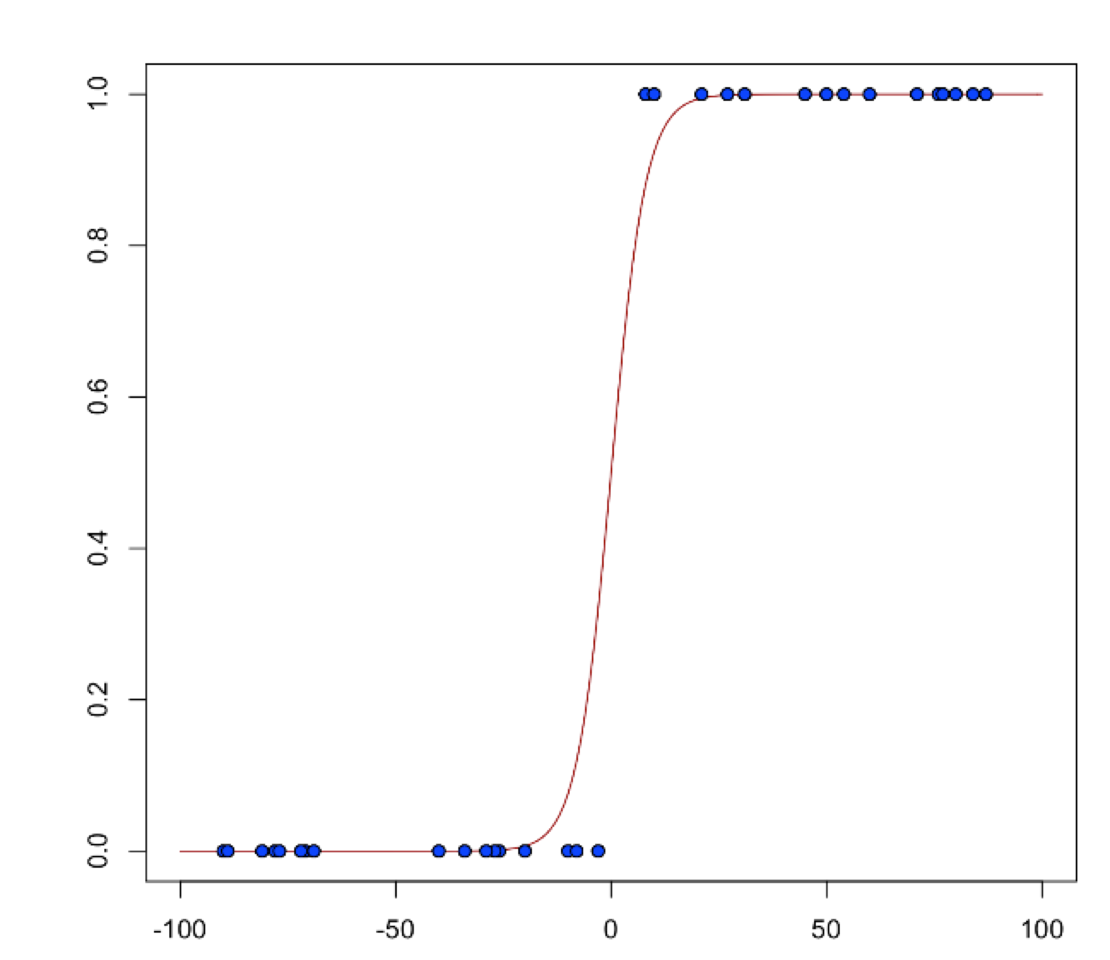
\includegraphics[scale=0.5]{images/scurve.png}
\end{figure}

\[ \hat{y} = Pr(y = 1|x) = {e^{x^T\beta + \beta_0} \over 1 + e^{x^T \beta + \beta_0} } \]

or alternatively:

\[log {\hat{y} \over 1- \hat{y}} = log{Pr(y=1|x) \over Pr(y=0|x)} = x^T \beta + \beta_0\]

The model is fitted by solving:
\[  \min\limits_{\beta,\beta_0} { {1 \over N}\sum\limits_{i=1}\limits^{N}(y_i (x_i^{T}\beta  + \beta_0) - log (1 + e^{x_i^{T}\beta  + \beta_0} )  + \lambda (\alpha \|\beta \|_1 + {1-\alpha \over 2}) \| \beta \|_2^2} \]

Deviance is -2 log likelihood:
\[D = -2\sum\limits_{i=1}\limits^{N}{(y log(\hat{y}) + (1 - y)log(1-\hat{y})  )}\]

\waterExampleInR

Using the prostate data set, build a binomial model that classifies if there is penetration of the prostatic
capsule (CAPSULE). Make sure the entries in the CAPSULE column are binary entries by using the \texttt{h2o.table()}
function. Change the regression by setting the family to binomial.

\begin{lstlisting}[style=R]
library(h2o)
h2o.init()
path = system.file("extdata", "prostate.csv", package = "h2o")
h2o_df = h2o.importFile(path)
is.factor(h2o_df$CAPSULE)
h2o_df$CAPSULE = as.factor(h2o_df$CAPSULE)
is.factor(h2o_df$CAPSULE)
binomial.fit = h2o.glm(y = "CAPSULE", x = c("AGE", "RACE", "PSA", "GLEASON"), training_frame = h2o_df, family = "binomial")
\end{lstlisting}

\subsubsection{Poisson Models}
Poisson regression is generally used in cases where the response represents counts and we assume errors have a
Poisson distribution. In general, it can be applied to any data where the response is non-negative.

When building a Poisson model, we usually model dependency of the mean on the log scale, i.e. canonical link is log
and prediction is:

\[\hat{y} = e^{x^T\beta + \beta_0}\]

The model is fitted by solving:

\[  \min\limits_{\beta,\beta_0} { {1 \over N}\sum\limits_{i=1}\limits^{N}(y_i (x_i^{T}\beta  + \beta_0) - e^{x_i^{T}\beta  + \beta_0})  + \lambda (\alpha \|\beta \|_1 + {1-\alpha \over 2}) \| \beta \|_2^2} \]

Deviance is:

\[D = -2\sum\limits_{i=1}\limits^{N}{(y log(\hat{y}) - y - \hat{y}}\]

\waterExampleInR

Load the Insurance data from the MASS library and import into H2O. Run a poisson model that predicts the number of
claims (Claims) based on the district of the policy holder (District), their age (Age), and the type of car they
own (Group).

\begin{lstlisting}[style=R]
library(h2o)
h2o.init()
library(MASS)
data(Insurance)

# Convert ordered factors into unordered factors.
# H2O only handles unordered factors today.
class(Insurance$Group) <- "factor"
class(Insurance$Age) <- "factor"

# Copy the R data.frame to an H2OFrame using as.h2o()
h2o_df = as.h2o(Insurance)
poisson.fit = h2o.glm(y = "Claims", x = c("District", "Group", "Age"), training_frame = h2o_df, family = "poisson")
\end{lstlisting}

\subsubsection{Gamma Models}
The gamma distribution is useful for modeling a positive continuous response variable, where the conditional
variance of the response grows with its mean but the coefficient of variation of the response $\sigma^2(x)/μ(x)$ is
constant for all x, i.e., it has a constant coefficient of variation.

It is usually used with inverse or log link, inverse is the canonical link.

The model is fitted by solving:

\[  \min\limits_{\beta,\beta_0} { {1 \over N}\sum\limits_{i=1}\limits^{N}{y_i \over (x_i^{T}\beta  + \beta_0)} - log({x_i^{T}\beta  + \beta_0})  + \lambda (\alpha \|\beta \|_1 + {1-\alpha \over 2}) \| \beta \|_2^2} \]

Deviance is:

\[D = -2\sum\limits_{i=1}\limits^{N}{log({y_i \over \hat{y}_i}) - {y_i - \hat{y}_i \over\hat{y}_i }}\]

\waterExampleInR

To change the link function from the default inverse function to the log link function, modify the \texttt{link}
argument.

\begin{lstlisting}[style=R]
library(h2o)
h2o.init()
path = system.file("extdata", "prostate.csv", package = "h2o")
h2o_df = h2o.importFile(path)
gamma.inverse <- h2o.glm(y = "DPROS", x = c("AGE","RACE","CAPSULE","DCAPS","PSA","VOL"), training_frame = h2o_df, family = "gamma", link = "inverse")
gamma.log <- h2o.glm(y="DPROS", x = c("AGE","RACE","CAPSULE","DCAPS","PSA","VOL"), training_frame = h2o_df, family = "gamma", link = "log")
\end{lstlisting}

\subsubsection{Tweedie Models}

TODO

%----------------------------------------------------------------------
%----------------------------------------------------------------------

\section{Building GLM Models in H2O}

H2O's GLM implementation presents a high-performance distributed algorithm, which scales linearly with the number
of rows and works extremely well for datasets with a limited number of active predictors.

\subsection{Classification vs. Regression}

GLM can produce both two categories of model, classification (binary classification only) and regression.  (Binary
classification in GLM is also called logistic regression.)

The data type of the response column determines the model category.  If the response data type is a categorical
(also called a factor or an enum) then a classification model will be created.  If the response column data type is
numeric (either integer or real), then a regression model will be created.

The following examples show how to coerce the data type of a column to a factor.

\bigskip
\waterExampleInR
\begin{lstlisting}[style=R]
library(h2o)
h2o.init()
path = system.file("extdata", "prostate.csv", package = "h2o")
h2o_df = h2o.importFile(path)
h2o_df$CAPSULE = as.factor(h2o_df$CAPSULE)
summary(h2o_df)
\end{lstlisting}

\waterExampleInPython
\begin{lstlisting}[style=python]
import h2o
h2o.init()
path = h2o.system_file("prostate.csv")
h2o_df = h2o.import_file(path)
h2o_df["CAPSULE"] = h2o_df["CAPSULE"].asfactor()
h2o_df.summary()
\end{lstlisting}

\subsection{Training and Validation Frames}

The word Frame in this context refers to an H2OFrame, the fundamental way of storing data in H2O's distributed memory.

\texttt{training\_frame} refers to a frame containing a training dataset.  All predictors and the response (as
well as offset and weights, if specified) must be part of this frame.

\texttt{validation\_frame} refers to an optional frame containing a validation dataset.  If specified, this 
frame must have the exact same columns as the training dataset.  Metrics are calculated on the validation dataset
for convenience purposes.

Note there are functions to calculate the same metrics after the model training completes for the case when a
validation dataset is not provided up front during training.

\subsection{Predictor and Response Variables}

Every model must specify its predictors and response.  Predictors and response are specified by the \texttt{x},
and \texttt{y} parameters.

\texttt{x} contains the list of column names or column indices referring to vectors from the training frame; it can
not contain periods.

\texttt{y} is a column name or index referring to a vector from the training frame.

\subsubsection{Categorical Variables}

If the response column is a categorical, then a classification model will be created.  GLM only supports binomial
classification, meaning the response column may only have two levels.

Predictor columns that are categorical may have more than two levels.

Users are encouraged to let GLM expand categorical columns itself.  GLM can take advantage of the categorical
column for better performance and memory utilization.

\textbf{Avoid one-hot encoding} categorical columns with many levels into many binary columns!  This is very
inefficient.  (This is especially true for Python users, who are used to expanding their categorical variables
manually for other frameworks.)

\subsection{Regularization Parameters}

See Section \ref{regularization} above for a detailed explanation.

To get the best possible model, we need to find the optimal values of the regularization parameters $\alpha$ and
$\lambda$.  To find the optimal values, H2O provides grid search over $\alpha$ and a special form of grid search
called ``lambda search over $\lambda$". The recommended way to find optimal regularization settings on H2O is to do
a grid search over a few $\alpha$ values with an automatic lambda search for each $\alpha$. Both are described
below in greater detail.

\subsubsection{alpha and lambda}

\texttt{alpha} controls the distribution between L1 (Lasso) and L2 (Ridge regression) penalties.  An \texttt{alpha} 
of 1.0 means only lasso, and an \texttt{alpha} of 0.0 means only ridge.

\texttt{lambda} controls the amount of regularization applied.  For a \texttt{lambda} value of 0.0, no 
regularization is applied, and the \texttt{alpha} parameter is ignored.  The default value for \texttt{lambda} is
calculated by H2O using a heuristic based on the training data.  If you let H2O calculate \texttt{lambda}, you can
see the chosen value in the model output.

\subsubsection{lambda search}

Lambda search is a special case of automatic and efficient grid search over lambda argument and is described in its
own section. Lambda search can be enabled by using the \texttt{lambda\_search = T} option. It can be further
parametrized by the \texttt{nlambdas} and \texttt{lambda\_min\_ratio} parameters.
\texttt{nlambdas} specifies the number of lambda values on the regularization path and \texttt{lambda\_min\_ratio} 
specifies the minimal lambda value to be computed as a ration of $\lambda_{max}$.

Lambda search can be enabled by using the \texttt{lambda\_search = T} option. It can be further parametrized by
the \texttt{nlambdas} and \texttt{lambda\_min\_ratio} parameters. When this option is enabled, H2O performs a
specialized grid search over the list of \texttt{nlambdas} $\lambda$ values, producing one model for each $\lambda$
value.

The $\lambda$-list is automatically generated as an exponentially decreasing sequence, going from $\lambda_{max}$,
the smallest $\lambda$ such that the solution is a model with all 0s, to $\lambda_{min} =
$ \textit{lambda\_min\_ratio} * $ \lambda_{max}$.

H2O computes $\lambda$-models sequentially and in decreasing order, warm-starting (using the previous solution as
the initial prediction) the model for $\lambda_k$ with the solution for $\lambda_{k-1}$. By warm-starting the
models, we get better performance: typically models for subsequent $\lambda$s are close to each other, so we need
only a few iterations per $\lambda$ (typically 2 or 3). We also achieve greater numerical stability, since models
with a higher penalty are easier to compute, so we start with an easy problem and then keep making only small
changes to it.

\textbf{Note:} \texttt{nlambda} and \texttt{lambda\_min\_ratio} also specify the relative distance of any two
 lambdas in the sequence. This is important when applying recursive strong rules, which are only effective if the
neighboring lambdas are ``close" to each other. The default values are \texttt{nlambda} = 100 and $\lambda_{min}
= \lambda_{max} 1e^{-4}$, which gives us the ratio of 0.912.  For best results when using strong rules, keep the
ratio close to the default.

\subsection{Family and Link}

Family and Link are both optional parameters. The default family is \texttt{Gaussian} and the default link is a
canonical link for the selected family. These are passed in as strings, e.g. \texttt{family=`gamma', link = `log'}.
While it is possible to select something other than a canonical link, doing so can lead to an unstable
computation. Recommended combinations are:

\begin{itemize}
\item \texttt{Gaussian} and \texttt{Log}
\item \texttt{Inverse, Gamma,} and \texttt{Log}
\end{itemize} 

\subsection{Handling Wide Data and Building Sparse Models}
\subsubsection{Solver Selection}
\subsubsection{Strong Rules for L1}

H2O's GLM employs strong rules (as described in \citetalias{strong}) to discard predictors that are likely to have
0 coefficients prior to model building. According to \citetalias{strong}, we can identify these predictors based on
a gradient with great accuracy. This provides very few false negatives and virtually no false positives in
practice, greatly reducing the computational complexity of model fitting and enabling it to run on wide datasets
with tens of thousands of predictors, provided that there is a limited number of active predictors.

When applying the strong rules, we evaluate the gradient at the starting solution, filter out inactive
coefficients, and fit a model using only a subset of the available predictors. Since strong rules may have false
positives (which are extremely rare in practice), we need to check the solution by testing the kkt conditions and
verify that all discarded predictors indeed have 0 coefficients.

\subsubsection{Stopping Criteria}

\subsection{Advanced Features}
\subsubsection{Standardizing Data}

\subsubsection{n-fold Cross Validation}

All validation values can be computed using either the training data set (the default option) or using N-fold
cross-validation (\texttt{nfolds $> 1$)}. When N-fold cross-validation is enabled, H2O randomly splits data into n
equally-sized parts, trains each of the n models on n-1 parts, and computes validation on the part that was not
used for training. The reported validation parameters are then obtained as follows:

\begin{itemize} 
\item Null deviance is sum of null deviances of n-models (each uses null model based on the subset of the data)
\item Residual deviance is sum of residual deviances of all n-models
\item AIC is based on log-likelihood, which is summed up similarly to deviance
\item AUC is based on ROC curve build  by summing up confusion matrices built for all n-models.
For each threshold, we get a confusion matrix that includes all the rows from the training set. However, each row
is classified exclusively by the model that did not contain that row in its training set. The computation of AUC is
the same as for a model without cross-validation.
\end{itemize}

\subsubsection{Grid Search}

\subsubsection{Grid Search Over Alpha}
Alpha search is not always needed and simply changing its value to 0.5 (or 0 or 1 if we only want Ridge or Lasso,
respectively) works in most cases. If $\alpha$ search is needed, usually only a few values are sufficient. Alpha
search is invoked by supplying a list of values for $\alpha$ instead of a single value. H2O then produces one model
per $\alpha$ value. The grid search computation can be done in parallel (depending on the cluster resources) and it
is generally more efficient than computing different models separately from R.

Use caution when including $\alpha=0$ or $\alpha=1$ in the grid search. $\alpha=0$ will produce a dense solution
and it can be really slow (or even impossible) to compute in large N situations. $\alpha=1$ has no L2 penalty, so
it is therefore less numerically stable and can be very slow as well due to slower convergence. In general, it is
safer to run with $alpha=1-\epsilon$ instead.

\subsubsection{Grid Search Over Lambdas}

While automatic lambda search is the preferred method, it is also possible to do a grid search over lambda values
by passing in vector of lambdas and disabling the lambda-search option. The behavior will be identical to lambda
search, except H2O will use a user-supplied list of lambdas instead (still capped at $\lambda_{max}$).

\subsubsection{Offsets}

\texttt{offset\_column} is an optional column name or index referring to a column in the training frame.

This column specifies a prior known component to be included in the linear predictor during training.

\subsubsection{Row Weights}

\texttt{weights\_column} is an optional column name or index referring to a column in the training frame.

This column specifies on a per-row basis the weight of that row.  If no weight column is specified, a default value
of 1 is used for each row.

\subsubsection{Coefficient Constraints}

Coefficient constraints allow you to set special conditions over the model coefficients. Currently supported
constraints are upper and lower bounds and the proximal operator interface, as described in \citetalias{prox}.

The constraints are specified as a frame with following vecs (matched by name; all vecs can be sparse):

\begin{itemize}
\item \texttt{names (mandatory)}  - coefficient names. 
\item \texttt{lower\_bounds (optional)} - coefficient lower bounds , must be $<= 0$
\item \texttt{upper\_bounds (optional)} - coefficient upper bounds , must be $>= 0$
\item \texttt{beta\_given (optional)} - specifies the given solution in proximal operator interface
\item \texttt{rho} (mandatory if \texttt{beta\_given} is specified, otherwise ignored) - specifies per-column L2 penalties on the distance from the given solution
\end{itemize}
 
The proximal operator interface allows you to run the GLM with a proximal penalty on a distance from a specified
given solution. There are many potential uses: for example, it can be used as part of an ADMM consensus algorithm
to obtain a unified solution over separate H2O clouds, or in Bayesian regression approximation.

\subsubsection{Proximal Operators}

%----------------------------------------------------------------------
%----------------------------------------------------------------------

\section{GLM Model Output}
\subsection{Coefficients and Normalized coefficients}
\subsection{Model outputs common to all families}
\subsubsection{Objective value}
\subsubsection{Scoring history}
\subsubsection{etc.}
\subsection{Additional model outputs for logistic regression (aka binomial classification)}
\subsubsection{AUC}
\subsubsection{etc.}
\subsection{Sanity checking the model}

%----------------------------------------------------------------------
%----------------------------------------------------------------------

\section{Making Predictions}
\subsection{Batch In-H2O predictions}
\subsection{Real-time low-latency predictions with the NanoFast scoring engine}

%----------------------------------------------------------------------
%----------------------------------------------------------------------

\section{R Use Case:  Logistic regression with Airline Dataset}

%----------------------------------------------------------------------
%----------------------------------------------------------------------

\section{Python Use Case:  Logistic regression with Airline Dataset}

%----------------------------------------------------------------------
%----------------------------------------------------------------------

Implementation Details
\subsection{Categorical Variables}

When applying linear models to datasets with categorical variables, the usual approach is to expand the
categoricals into a set of binary vectors, with one vector per each categorical level (e.g. by calling
{\texttt{model.matrix}} in R). H2O performs similar expansions automatically and no prior changes to the dataset
are needed. Each categorical column is treated as a set of sparse binary vectors.

\subsubsection{Largest Categorical Speed Optimization}

Categoricals have special handling during GLM computation as well. When forming the gram matrix, we can take
advantage of the fact that columns belonging to the same categorical never co-occur and the gram matrix region
belonging to these columns will not have any non-zero elements outside of the diagonal. We can thus keep it in
sparse representation, taking only O(N) elements instead of O(N*N). Furthermore, the complexity of Choelsky
decomposition of a matrix that starts with a diagonal region can be greatly reduced. H2O's GLM exploits these two
facts to handle the largest categorical ``for free". Therefore, when analyzing the performance of GLM in the
equation expressed above, we can subtract the size of the largest categoricals from the number of predictors.

$$N = \sum_{c \in C} (\|c.domain\|) - \arg\max_{c \in C} \|c.domain\| + \|Nums\| $$

\subsection{Performance}

The implementation is based on iterative re-weighted least squares with an ADMM inner solver (as described
in \citetalias{admm}) to deal with the L1 penalty. Every iteration of the algorithm consists of following steps:

\begin{enumerate} 
\item Generate weighted least squares problem based on previous solution, i.e. vector of weights w and response z 
\item Compute the weighted gram matrix $X^TWX$ and $X^Tz$ vector
\item Decompose the gram matrix (Cholesky decomposition) and apply ADMM solver to solve the L1 penalized least squares problem
\end{enumerate}

Steps 1 and 2 are performed distributively and step 3 is computed in parallel on a single node. We can thus
characterize the computational complexity and scalability of dataset with M observations and N columns (predictors)
on a cluster with n nodes with p CPUs each as follows:

\[ O({MN^2 \over pn} + {N^3 \over p})\]

And the overall memory cost is given by:

\[ O(MN + N^2pn)\]

If $M >> N$, the second term is not needed and the algorithm scales linearly both in the number of nodes and the
number of CPUs per node. However, the equation above also implies that our algorithm is limited in the number of
predictors it can handle, since the size of the Gram matrix grows quadratically due to a memory and network
throughput issue with the number of predictors and its decomposition cost grows as the cube of the number of
predictors (which is a computational cost issue). In many cases, H2O can work around these limitations due to its
handling of categoricals and by employing strong rules to filter out inactive predictors.

\subsection{Handling Data with Many Predictors}
\subsection{Data Corner Cases}

%----------------------------------------------------------------------
%----------------------------------------------------------------------

\section{OLD}

\subsection{H2O GLM Model Output}
The detailed output of the GLM model varies depending on the distribution used for the model. In general, there is
shared output for all Families: Coefficients \& Normalized Coefficients, Validation, and Prediction. We'll cover
the model output from an R user's point of view.

First, let's build a simple GLM on a small dataset and see what we get out:

\begin{lstlisting}[style=R]
library(h2o)

# Initialize H2O
h <- h2o.init()

# path to the data
data.bucket <- "https://raw.githubusercontent.com/h2oai/h2o/master/smalldata"
data.path <- paste(data.bucket, "/logreg/prostate_train.csv", sep = "")

# import the data from the url
hex <- h2o.importFile(h, data.path)

# build a binomial regression
m <- h2o.glm(x = 3:9, y = 2, data = hex, family = "binomial")  
# no other features tweaked... yet
\end{lstlisting}

The default \texttt{show} of this model has the following output:

\begin{lstlisting}[style=output]
IP Address: 127.0.0.1 
Port      : 54321 
Parsed Data Key: prostate_train.hex 

GLM2 Model Key: GLMModel__8b954fd700d924f3e9dee8717b8246ef

Coefficients:
      AGE      RACE     DPROS     DCAPS       PSA       VOL   GLEASON Intercept 
 -0.07668  -0.10320   0.59479   0.13549   0.43841  -0.22215   1.19657  -0.49458 

Normalized Coefficients:
      AGE      RACE     DPROS     DCAPS       PSA       VOL   GLEASON Intercept 
 -0.07668  -0.10320   0.59479   0.13549   0.43841  -0.22215   1.19657  -0.49458 

Degrees of Freedom: 304 Total (i.e. Null);  297 Residual
Null Deviance:     412.1
Residual Deviance: 301.9  AIC: 317.9
Deviance Explained: 0.26733 
 Best Threshold: 0.44

Confusion Matrix:
        Predicted
Actual   false true Error
  false    147   34 0.188
  true      32   92 0.258
  Totals   179  126 0.216

AUC =  0.8318927 (on train) 
\end{lstlisting}

Briefly, the output contains the IP address and port number of the H2O cluster where the model was trained. It
includes the data key, the model key, the coefficients, and some model metrics. Let's look at these in detail.

\subsubsection{Coefficients \& Normalized Coefficients}

Coefficients are the predictor weights (i.e. the actual model used for prediction).  If the \texttt{standardize}
option is enabled, H2O returns another set of coefficients, the normalized coefficients. These are the predictor
weights of the standardized data and are included only for informational purposes (e.g. to compare relative
variable importance). In this case, the coefficients are obtained from the normalized coefficients
by \textbf{reversing} the data standardization process (de-scaled, with the intercept adjusted by an added offset)
so that they can be applied to data in its original form (i.e. no standardization prior to scoring). \textbf{Note:}
These are \textbf{not} the same as coefficients of a model built on non-standardized data.

\subsubsection{Validation}

By default, H2O's GLM generates additional models with 1/10 of the original data to performs 10-fold
cross-validation. This will provide a quick idea of how the model will generalize. However, it's always best to
evaluate the model using some holdout data.

\subsubsection{Generating Predictions}

The following R code generates predictions:

\begin{lstlisting}[style=R]
test.path <- paste(data.bucket, "/logreg/prostate_test.csv", sep = "")

# import the data from the url
test <- h2o.importFile(h, test.path)

# generate the predictions
predictions <- h2o.predict(m, test)

# look at the first 6 entries of predictions
predictions

# generate the model metrics
h2o.performance(data=predictions[,3], reference=test[,1])
\end{lstlisting}

\subsection{Categorical Variables}

\subsection{Cross-Validation}

\subsection{Selecting Regularization Parameters}

\subsubsection{Lambda Search}  %%can this be combined with 6.1.3 Lambda Search above? or referenced? seems to contain duplicate info 
    

\subsection{Strong Rules} %TODO add references

\subsection{Performance Characteristics}

%----------------------------------------------------------------------
%----------------------------------------------------------------------

\section{Use case: Classification with Airline data}

\subsection{Airline dataset overview} 

Download the Airline dataset here: {\url{https://github.com/h2oai/h2o/blob/master/smalldata/airlines/allyears2k_headers.zip}}.

Save the .csv file to your working directory by clicking  "View Raw."  Before running the Airline demo, we'll review how to load data with H2O. 

\subsubsection{Loading data} \label{2.5}

Loading a dataset in R for use with H2O is slightly different from the usual methodology because we must convert our datasets into \texttt{H2OParsedData} objects. In this example, we will use a toy weather dataset that is available here: {\url{https://raw.githubusercontent.com/h2oai/h2o/master/smalldata/weather.csv}}. 

First, load the data to your current working directory in your R Console (do this for any future dataset downloads), and then run the following command:
\begin{lstlisting}[style=R]
weather.hex = h2o.uploadFile(localH2O, path = "weather.csv", header = TRUE, sep = ",", key = "weather.hex")
\end{lstlisting}
\bigskip

To see a quick summary of the data, run the following command:
\begin{lstlisting}[style=R]
summary(weather.hex)
\end{lstlisting}

\subsection{Performing a trial run} \label{3.2}
Returning to the Airline dataset demo, we first load the dataset into H2O and select the variables we want to use to predict a chosen response. For example, we can model if flights are delayed based on the departure's scheduled day of the week and day of the month.

\begin{lstlisting}[style=R]
library(h2o)
localH2O = h2o.init(nthreads = -1)
#Load the data and prepare for modeling
air_train.hex = h2o.uploadFile(localH2O, path = "~/Downloads/AirlinesTrain.csv", header = TRUE, sep = ",", key = "airline_train.hex")
air_test.hex = h2o.uploadFile(localH2O, path = "~/Downloads/AirlinesTest.csv", header = TRUE, sep = ",", key = "airline_test.hex")
x = c("fYear", "fMonth", "fDayofMonth", "fDayOfWeek", "UniqueCarrier", "Origin", "Dest", "Distance")
y = "IsDepDelayed"
\end{lstlisting}

Now we train the GLM model:

\begin{lstlisting}[style=R]
airline.glm <- h2o.glm(x=x, y=y, data=air_train.hex, key = "glm_model", family="binomial", lambda_search = TRUE, return_all_lambda = TRUE, use_all_factor_levels = TRUE, variable_importances = TRUE)
\end{lstlisting}

\subsubsection{Extracting and handling the results} \label{3.2.1}

We can extract the parameters of our model, examine the scoring process, and make predictions on new data.

\begin{lstlisting}[style=R]
# Predict on GLM model
best_glm = airline.glm@models[[airline.glm@best_model]]
air.results = h2o.predict(object = best_glm, newdata = air_test.hex)

# Check performance and AUC
perf = h2o.performance(air.results$YES, air_test.hex$IsDepDelayed )
print(perf)
perf@model$auc

# Show distribution of predictions with quantile
quant = quantile.H2OParsedData(air.results$YES)

# Extract strongest predictions
top.air <- h2o.assign(air.results[air.results$YES > quant["75%"]], key="top.air")
top.air
\end{lstlisting}

Once we have a satisfactory model, the \texttt{h2o.predict()} command can be used to compute and store predictions on the new data, which can then be used for further tasks in the interactive modeling process.
\begin{lstlisting}[style=R]
#Perform classification on the held out data
prediction = h2o.predict(object = best_glm, newdata=air_test.hex)

#Copy predictions from H2O to R
pred = as.data.frame(prediction)
head(pred)
\end{lstlisting}

\subsection{Web interface} \label{3.3}
H2O R users have access to an intuitive web interface for H2O, Flow, to mirror the model building process in R. After loading data or training a model in R, point your browser to your IP address and port number (e.g., localhost:12345) to launch the web interface. From here, you can click on \textsc{Admin} $>$ \textsc{Jobs} to view specific details about your model. You can also click on \textsc{Data} $>$ \textsc{List All Frames} to view all current H2O frames. 

\subsubsection{Variable importances} \label{3.3.1}
The variable importances feature can be enabled with the argument \texttt{variable\_importances=TRUE}.This feature allows us to view the absolute and relative predictive strength of each feature in the prediction task. From R, you can access these strengths with the command \texttt{air.model@model\$varimp}. You can also view a visualization of the variable
importances on the web interface.

\subsubsection{Java model} %%should this be replaced with instructions for Java POJOs? 
Java models are currently not available for GLM.
To download the model, 
\begin{enumerate}
\item Open the terminal window. 
\item Create a directory where the model will be saved.
\item Set the new directory as the working directory.
\item Follow the curl and java compile commands displayed in the instructions at the top of the Java model.
\end{enumerate}
\newpage

%----------------------------------------------------------------------
%----------------------------------------------------------------------

\section{H2O Community Resources}
\begin{singlespacing}

For more information about H2O, visit the following open-source sites:

\begin{tabular}{l l}
{\textbf{H2O Full Documentation}}: & \url{http://docs.h2o.ai} \\
\\
{\textbf{H2O-3 Github Repository}}: & \url{https://github.com/h2oai/h2o-3} \\
\\
{\textbf{Open-source discussion forum}}: & \href{mailto:h2ostream@googlegroups.com}{\texttt{h2ostream@googlegroups.com}} \\
& {\small{\url{groups.google.com/d/forum/h2ostream}}} \\
\\
{\textbf{Issue tracking}}: & \url{http://jira.h2o.ai}
\end{tabular}

\end{singlespacing}
\bigskip



%----------------------------------------------------------------------
%----------------------------------------------------------------------

\section{Appendix: Parameters}
\begin{itemize}
\item \texttt{x}: A vector containing the names of the predictors to use while building the GLM model. No default.
\item \texttt{y}: A character string or index that represents the response variable in the model. No default.
\item \texttt{training\_frame}: An \texttt{H2OFrame} object containing the variables in the model. 
\item \texttt{model\_id}: (Optional) The unique ID assigned to the generated model. If not specified, an ID is generated automatically.
\item \texttt{validation\_frame}: An \texttt{H2OParsedData} object containing the validation dataset used to construct confusion matrix. If  blank, the training data is used by default.
\item \texttt{max\_iterations}: A non-negative integer specifying the maximum number of iterations. 
\item \texttt{beta\_epsilon}: A non-negative number specifying the magnitude of the maximum difference between the coefficient estimates from successive iterations. Defines the convergence criterion. 
\item \texttt{solver}: A character string specifying the solver used: either \texttt{IRLSM}, which supports more features, or \texttt{L\_BFGS}, which scales better for datasets with many columns. 
\item \texttt{standardize}: A logical value that indicates whether the numeric predictors should be standardized to have a mean of 0 and a variance of 1 prior to model training. 
\item \texttt{family}: A description of the error distribution and corresponding link function to be used in the model. The following options are supported: \texttt{gaussian, binomial, poisson, gamma,} or \texttt{tweedie}. When a model is specified as Tweedie, users must also specify the appropriate Tweedie power. No default. %%need to specify `tweedie_variance_power` and `tweedie_link_power`??
\item \texttt{link}: The link function relates the linear predictor to the distribution function. The default is the canonical link for the specified family. The full list of supported links: 
	\begin{itemize}
\item	{\textbf {gaussian}}: identity, log, inverse 
\item {\textbf{binomial}}: logit, log 
\item {\textbf{poisson}}: log, identity
\item {\textbf{gamma}}: inverse, log, identity
\item {\textbf{tweedie}}: tweedie 
	\end{itemize}
\item \texttt{tweedie\_variance\_power}: A numeric specifying the power for the variance function when \texttt{family = "tweedie"}. 
\item \texttt{tweedie\_link\_power}: A numeric specifying the power for the link function when \texttt{family = "tweedie"}. 
\item \texttt{alpha}: The elastic-net mixing parameter, which must be in $[0,1]$. The penalty is defined to be $P(\alpha,\beta) = (1-\alpha)/2||\beta||_2^2 + \alpha||\beta||_1 = \sum_j [(1-\alpha)/2 \beta_j^2 + \alpha|\beta_j|] $ so \texttt{alpha=1} is the lasso penalty, while \texttt{alpha=0} is the ridge penalty. Default is 0.5.
\item \texttt{prior}: (Optional) A numeric specifying the prior probability of class 1 in the response when \texttt{family = "binomial"}. The default value is the observation frequency of class 1. 
\item \texttt{lambda}: A non-negative value representing the shrinkage parameter, which multiplies $P(\alpha,\beta)$ in the objective. The larger lambda is, the more the coefficients are shrunk toward zero (and each other). When the value is 0, no elastic-net penalty is applied and ordinary generalized linear models are fit. Default is 1e-05.
\item \texttt{lambda\_search}: A logical value indicating whether to conduct a search over the space of lambda values, starting from the max lambda, given lambda will be interpreted as the min. lambda. Default is false.
\item \texttt{nlambdas}: The number of lambda values when \texttt{lambda\_search = TRUE}. Default is -1.
\item \texttt{lambda\_min\_ratio}: Smallest value for lambda as a fraction of lambda.max, the entry value, which is the smallest value for which all coefficients in the model are zero. If the number of observations is greater than the number of variables then \texttt{lambda\_min\_ratio = 0.0001}; if the number of observations is less than the number of variables then \texttt{lambda\_min\_ratio = 0.01}. Default is -1.0.
\item \texttt{nfolds}: Number of folds for cross-validation. If \texttt{nfolds >=2}, then \texttt{validation\_frame} must remain blank. Default is 0. %%validation_frame = correct? just says "validation" in R doc...
\item \texttt{fold\_column}: (Optional) Column with cross-validation fold index assignment per observation. 
\item \texttt{fold\_assignment}: Cross-validation fold assignment scheme, if \texttt{fold\_column} is not specified. The following options are supported: \texttt{AUTO, Random,} or \texttt{Modulo}. 
\item \texttt{keep\_cross\_validation\_predictions}: Specify whether to keep the predictions of the cross-validation models. 
\item \texttt{beta\_constraints}: A data frame or \texttt{H2OParsedData} object with the columns \texttt{["names", "lower\_bounds", "upper\_bounds", "beta\_given"]}, where each row corresponds to a predictor in the GLM. \texttt{"names"} contains the predictor names, \texttt{"lower\_bounds"/"upper\_bounds"} are the lower and upper bounds (respectively) of the beta, and \texttt{"beta\_given"} is a user-specified starting value. 
\item \texttt{offset\_column}: Specify the offset column. Note: Offsets are per-row “bias values” that are used during model training. For Gaussian distributions, they can be seen as simple corrections to the response (y) column. Instead of learning to predict the response (y-row), the model learns to predict the (row) offset of the response column. For other distributions, the offset corrections are applied in the linearized space before applying the inverse link function to get the actual response values. 
\item \texttt{weights\_column}: Specify the weights column. Note: Weights are per-row observation weights. This is typically the number of times a row is repeated, but non-integer values are supported as well. During training, rows with higher weights matter more, due to the larger loss function pre-factor.
\item \texttt{intercept}: Logical; includes a constant term (intercept) in the model. If there are factor columns in your model, then the intercept must be included. %% <--- still true? copied from `has_intercept`
\end{itemize}
%Additional: 
%Strong Rules Enables: Uses strong rules to filter out inactive columns. Default is true.
%Ignored_cols: No default.
%Non-negative: Restricts coefficients to be non-negative. Default is false.
%parallelism: @Is this just a python thing?

\newpage

\begin{thebibliography}{9}

\bibitem{glmnet} 
Jerome Friedman, Trevor Hastie, and Rob Tibshirani.
\textbf{Regularization Paths for Generalized Linear Models via Coordinate Descent}.
April 29, 2009

\bibitem{strong} 
  Robert Tibshirani, Jacob Bien, Jerome Friedman, Trevor Hastie, Noah Simon, Jonathan Taylor, and Ryan J. Tibshirani. 
  \textbf{Strong Rules for Discarding Predictors in Lasso-type Problems}.
  J. R. Statist. Soc. B, vol. 74, 2012.
\bibitem{elastic}
Hui Zou and Trevor Hastie
\textbf{Regularization and variable selection via the elastic net}. 
J. R. Statist. Soc. B (2005) 67, Part 2, pp. 301-320

\bibitem{lasso}
Robert Tibshirani.
\textbf{Regression Shrinkage and Selection via the Lasso}
Journal of the Royal Statistical Society. Series B (Methodological), Volume 58, Issue 1 (1996), 267-288

\bibitem{admm}
S. Boyd, N. Parikh, E. Chu, B. Peleato, and J. Eckstein.
\textbf{Distributed Optimization and Statistical Learning via the Alternating Direction Method of Multipliers}. 
Foundations and Trends in Machine Learning, 3(1):1–122, 2011. (Original draft posted November 2010.)

\bibitem{prox}
N. Parikh and S. Boyd.\
\textbf{Proximal Algorithms}.
Foundations and Trends in Optimization, 1(3):123-231, 2014.

\bibitem{git}
{\url{http://github.com/h2oai/h2o.git}}

\bibitem{docs}
{\url{http://docs.h2o.ai}}

\bibitem{stream}
{\url{https://groups.google.com/forum/#!forum/h2ostream}}

\bibitem{h2o}
{\url{http://h2o.ai}}

\bibitem{jira}
{\url{https://0xdata.atlassian.net/secure/Dashboard.jspa}}
\end{thebibliography}

\end{document}
